\documentclass[12pt,a4paper]{article}
\usepackage[warn]{mathtext}
\usepackage[utf8]{inputenc}
\usepackage[english,russian]{babel}
\usepackage{amsmath}
\usepackage{amssymb}
\usepackage{latexsym}
\usepackage{svg}
\usepackage{pgfplots}
\pgfplotsset{compat=1.9}

\usepackage{listings}

\usepackage{color}

\definecolor{dkgreen}{rgb}{0,0.6,0}
\definecolor{gray}{rgb}{0.5,0.5,0.5}
\definecolor{mauve}{rgb}{0.58,0,0.82}

\lstset{ %
	language=C++,                % Язык программирования 
	numbers=left,                   % С какой стороны нумеровать
	stepnumber=1,                   % Шаг между линиями. Если 1, то будет пронумерована каждая строка
	frame=single,	
}
\usepackage[left=2cm,right=2cm,
top=2cm,bottom=2cm,bindingoffset=0cm]{geometry}

\usepackage{sverb}
\usepackage{graphicx}
\usepackage{pdfpages}
\usepackage[absolute,overlay]{textpos}

\numberwithin{equation}{section}

\begin{document}
	\begin{titlepage}
		\begin{textblock*}{13cm}(0cm,0cm)
			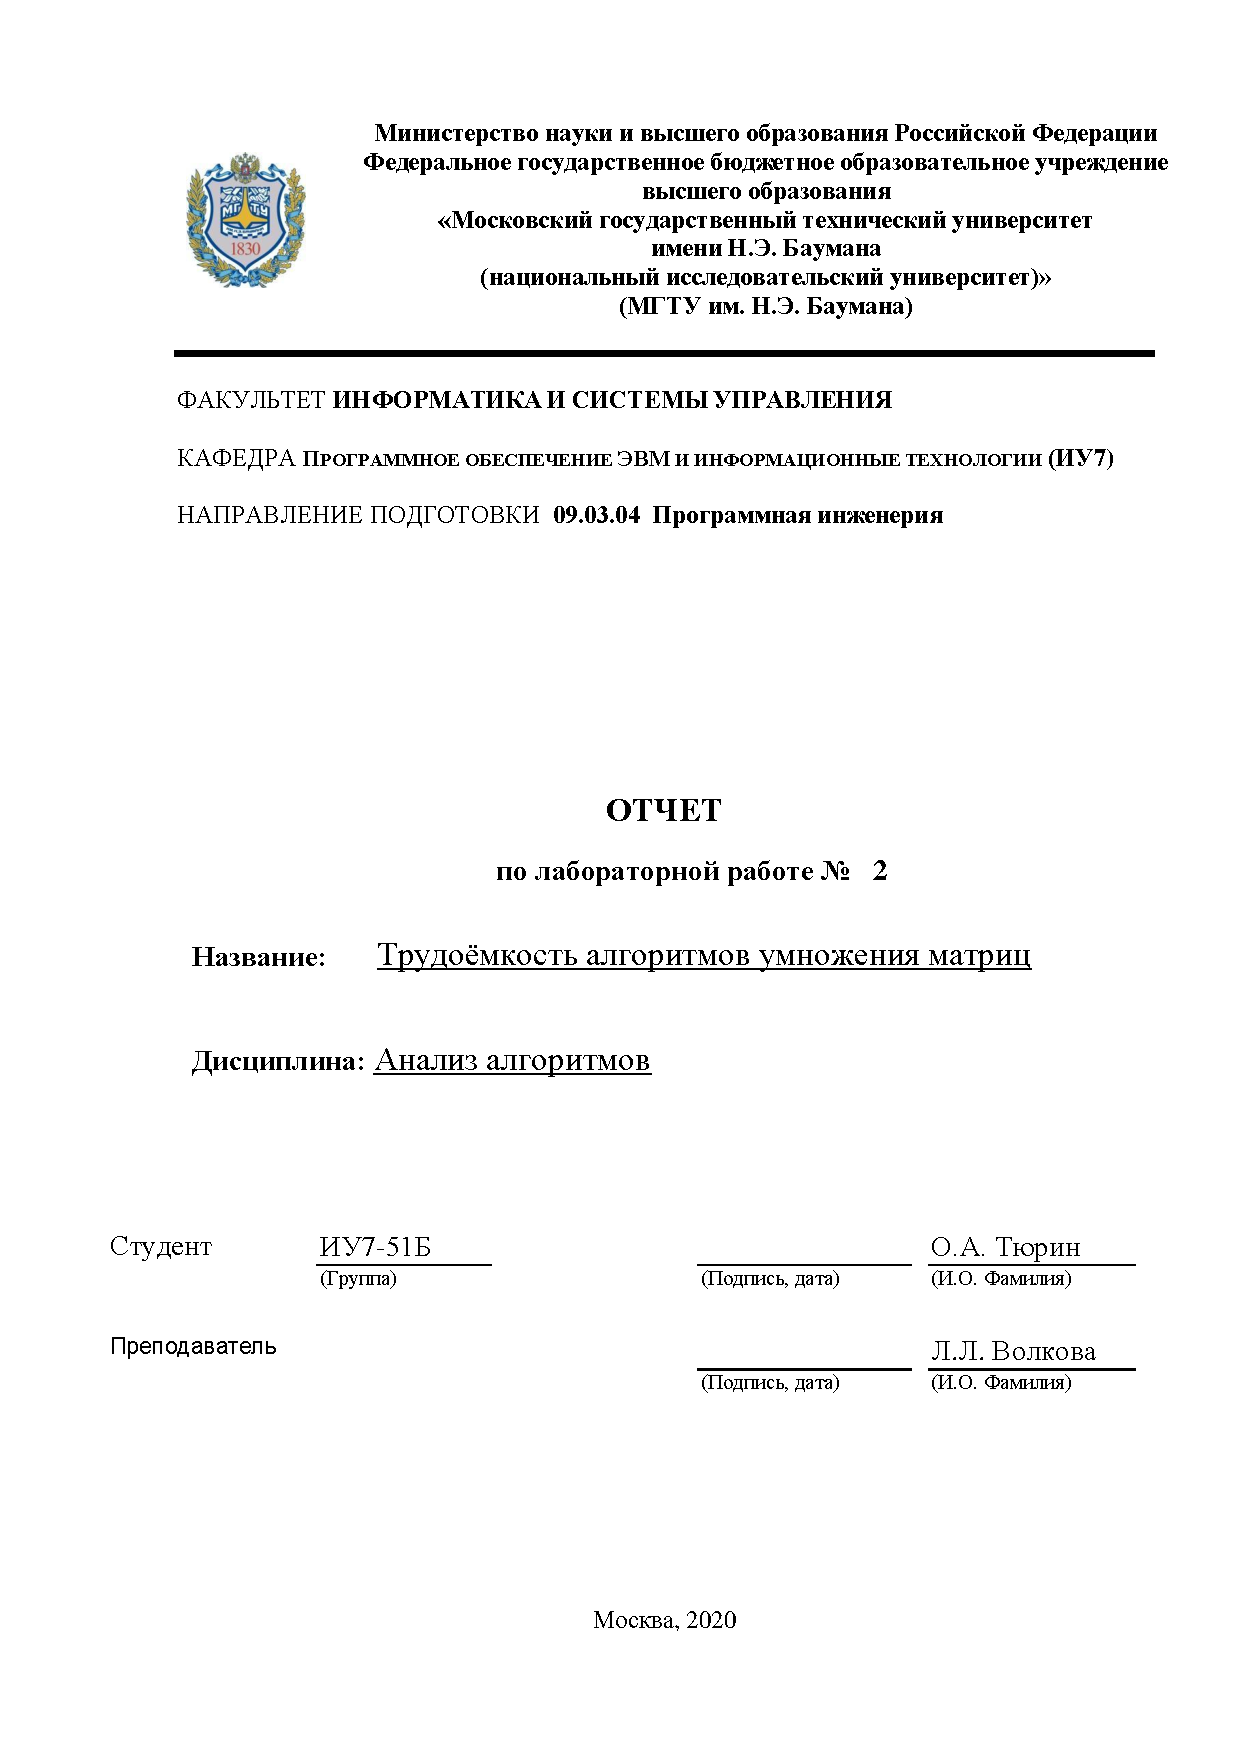
\includegraphics{reportTitle}
		\end{textblock*}
	\end{titlepage}
\hspace{0pt}
\clearpage
%	\begin{titlepage}
%		\centering
%		\Huge Лабораторная работа №1 по курсу \\\textbf{"Анализ алгоритмов"}\\
%		Тема: Расстояния Левенштейна и Дамерау-Левенштейна\\
%		\vspace{\baselineskip}
%		\Large Работу выполнил: Тюрин О.А. ИУ7-51Б\\
%		Преподаватели: Волкова Л.Л, Строганов Ю.В.
%		\vfill
%		Москва, 2020 г.		
%	\end{titlepage}
\tableofcontents
\clearpage

\addcontentsline{toc}{section}{Введение}
%//////////////////////////////////////////////////////////////////
\section*{\Huge Введение}
\qquad Целью данной лабораторной работы является исследование методов умножения матриц, получение практического навыка синтезации алгоритма и рассчёт сложности алгоритмов. Помимо обычного метода будут рассмотрены алгоритм Винограда умножения матриц и оптимизированный алгоритм Винограда умножения матриц.\\
\qquad Применение: умножение матрицы на вектор используется в графике для поворота образа.\\
\qquad Задачи для данной ЛР:
\begin{itemize}
\item изучение алгоритмов умножения матриц: стандартный и алгоритм Винограда;
\item оптимизировать алгоритм Винограда умножения матриц;
\item дать теоретическую оценку всем трём алгоритмам;
\item релизовать все три алгоритма на одном из языков программирования;
\item эксперементально подтвердить различия во временной эффективности всех трёх алгоритмов при помощи разработанного программного обеспечения на материале замеров процессорного времени выполнения реализации на варьирущихся размерностях матриц.
\end{itemize}
\clearpage

\section{Аналитическая часть}
\qquad Матрица — математический объект, записываемый в виде прямоугольной таблицы элементов. Умножение матриц — одна из основных операций над матрицами. Матрица, получаемая в результате операции умножения, называется произведением матриц. Матрицы A и B могут быть перемножены, если они \textbf{совместимы} в том смысле, что число столбцов матрицы A равно числу строк B.

\subsection{Описание алгоритмов}
\qquad В данном разделе будет описан каждый из исследуемых алгоритмов.

\subsubsection{Обычный алгоритм умножения матриц}
\qquad Пусть даны две прямоугольные матрицы А и В размеров $[M * N]$ и $[N * Q]$ соответственно.
\begin{equation*}
A = \left(
\begin{array}{cccc}
a_{11} & a_{12} & \ldots & a_{1n}\\
a_{21} & a_{22} & \ldots & a_{2n}\\
\vdots & \vdots & \ddots & \vdots\\
a_{m1} & a_{m2} & \ldots & a_{mn}
\end{array}
\right)
\end{equation*}

\begin{equation*}
B = \left(
\begin{array}{cccc}
b_{11} & b_{12} & \ldots & a_{1q}\\
b_{21} & b_{22} & \ldots & a_{2q}\\
\vdots & \vdots & \ddots & \vdots\\
b_{n1} & a_{n2} & \ldots & a_{nq}
\end{array}
\right)
\end{equation*}

\qquad В результате произведения матриц A и B получим матрицу C размера $[M *  Q]$, в которой:
\begin{equation}
	c_{i,j} = \sum\limits_{r=1}^N a_{i,r}\cdot b_{r,j}.
\end{equation}

\newpage

\subsubsection{Алгоритм Винограда}
\qquad Основной целью алгоритма Винограда является сокращение доли умножений в самом затратном участке кода.

\qquad Рассмотри два вектора:
\begin{equation*}
A = \left(
\begin{array}{cccc}
a_{1} & a_{2} & a_{3} & a_{4}
\end{array}
\right)
\end{equation*}

\begin{equation*}
B = \left(
\begin{array}{c}
b_{1}\\
b_{2}\\
b_{3}\\
b_{4}\\
\end{array}
\right)
\end{equation*}

\begin{equation}
	A * B = a_{1} * b_{1} + a_{2} * b_{2} + a_{3} * b_{3} + a_{4} * b_{4}
\end{equation}
Но в то же время:\\
\begin{equation}
	A * B = (a_{1} + b_{2}) * (a_{2} + b_{1}) + (a_{3} + b_{4}) * (a_{4} + b_{3}) - a_{1}*a_{2} - a_{3}*a_{4} - b_{1}*b_{2} - b_{3}*b_{4}
\end{equation}
\qquad В данном примере значения  $b_{1}*b_{2}, b_{3}*b_{4}$ можно вычислить заранее и использовать при каждом умножении на строку матрицы А. Значения $a_{1}*a_{2}, a_{3}*a_{4}$ также можно вычислить заранее и использовать при каждом умножении на столбец матрицы B.
%//////////////////////////////////////////////////////////////////
\subsubsection{Оптимизированный алгоритм Винограда}
Для оптимизации алгоритма Винограда могут использоваться такие стратегии, как:
\begin{itemize}
	\item предварительные вычисления повторяющихся одинаковых действий;
	\item использование более быстрых операций при вычислении (такие, как смещение битов вместо умножения или деления на 2);
	\item уменьшения количества повторных проверок;
	\item использование аналогичных конструкций, уменьшающих трудоёмкость операций (к примеру, замена сложения с 1 на инкремент).
\end{itemize}
\addcontentsline{toc}{subsection}{Вывод}
\section*{Вывод}
\qquad Было рассмотрено теоретическое описание исследуемых алгоритмов: Обычный алгоритм умноженмя и алгоритм Винограда.
\clearpage

\section{Конструкторская часть}
\textbf{Требования к вводу:} на вход подаются размерности каждой из матриц и сами матрицы.\\\\
\textbf{Требования к программе:}\\
\begin{itemize}
\item корректное умножение двух матриц;
\item программа должна корректно обрабатывать ситуацию несовместности двух матриц.
\end{itemize}
\clearpage
\subsection{Разработка алгоритмов} % Сюда схемы алгоритмов
\qquad В данном разделе представлены схемы реализуемых алгоритмов.
\subsubsection{Схема алгоритмов}
На рисунке 1.1 представлена схема алгоритма тривиального умножения матриц.
\begin{center}	
	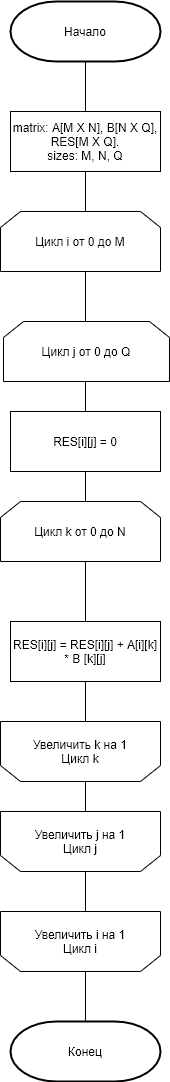
\includegraphics[width=0.18\linewidth]{src/schemas/mult_trivial}\\
	Рис. 1.1: Схема алгоритма тривиального умножения матриц
\end{center}
\clearpage
На рисунке 1.2 представлена схема алгоритма Винограда.
\begin{center}	
	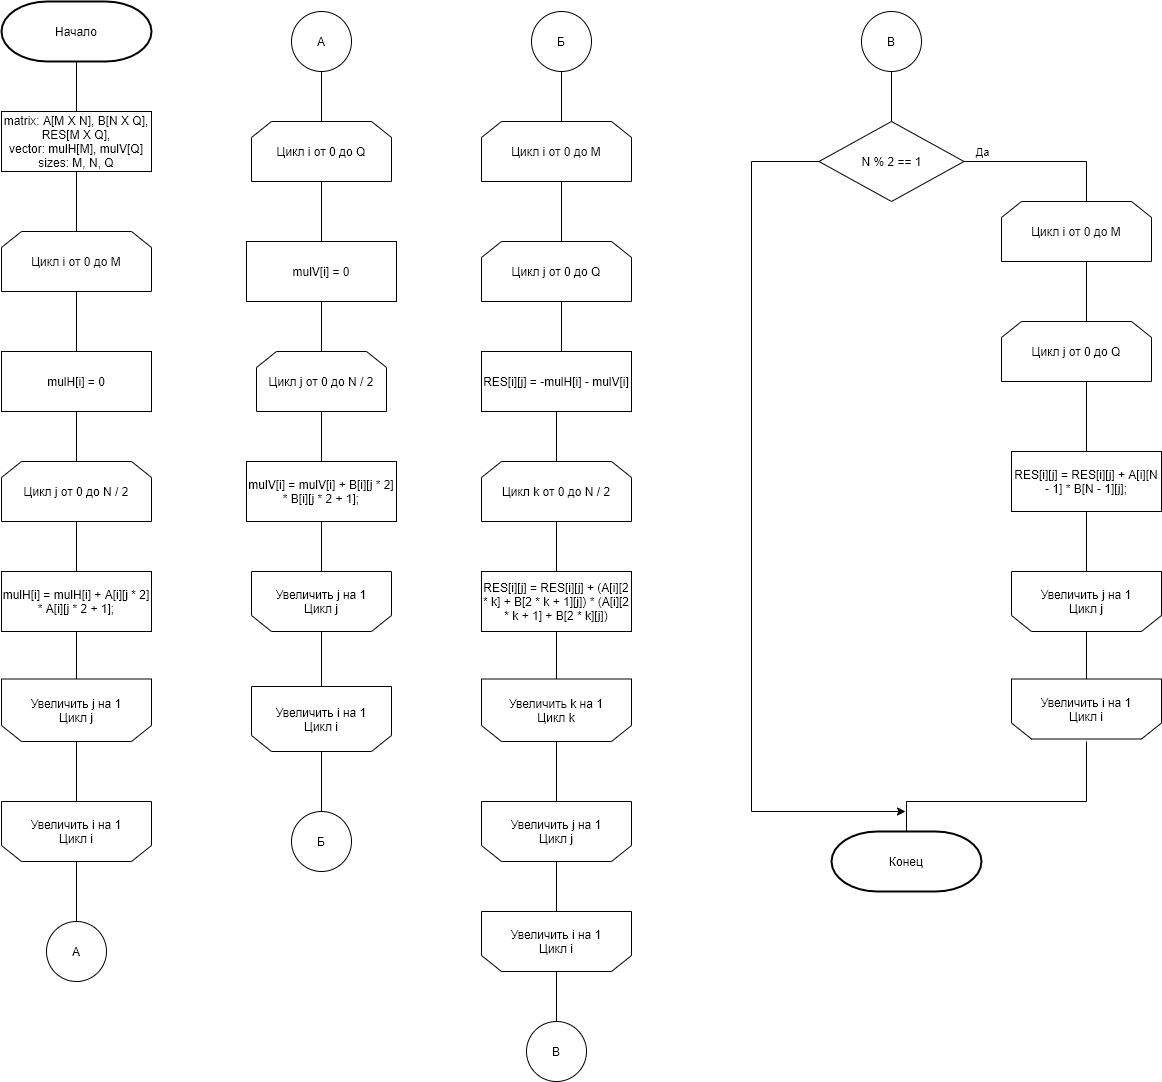
\includegraphics[width=1\linewidth]{src/schemas/vinograd_default}\\
	Рис. 1.2: Схема алгоритма Винограда
\end{center}
\clearpage
На рисунке 1.3 представлена схема улучшенного алгоритма Винограда.
\begin{center}
	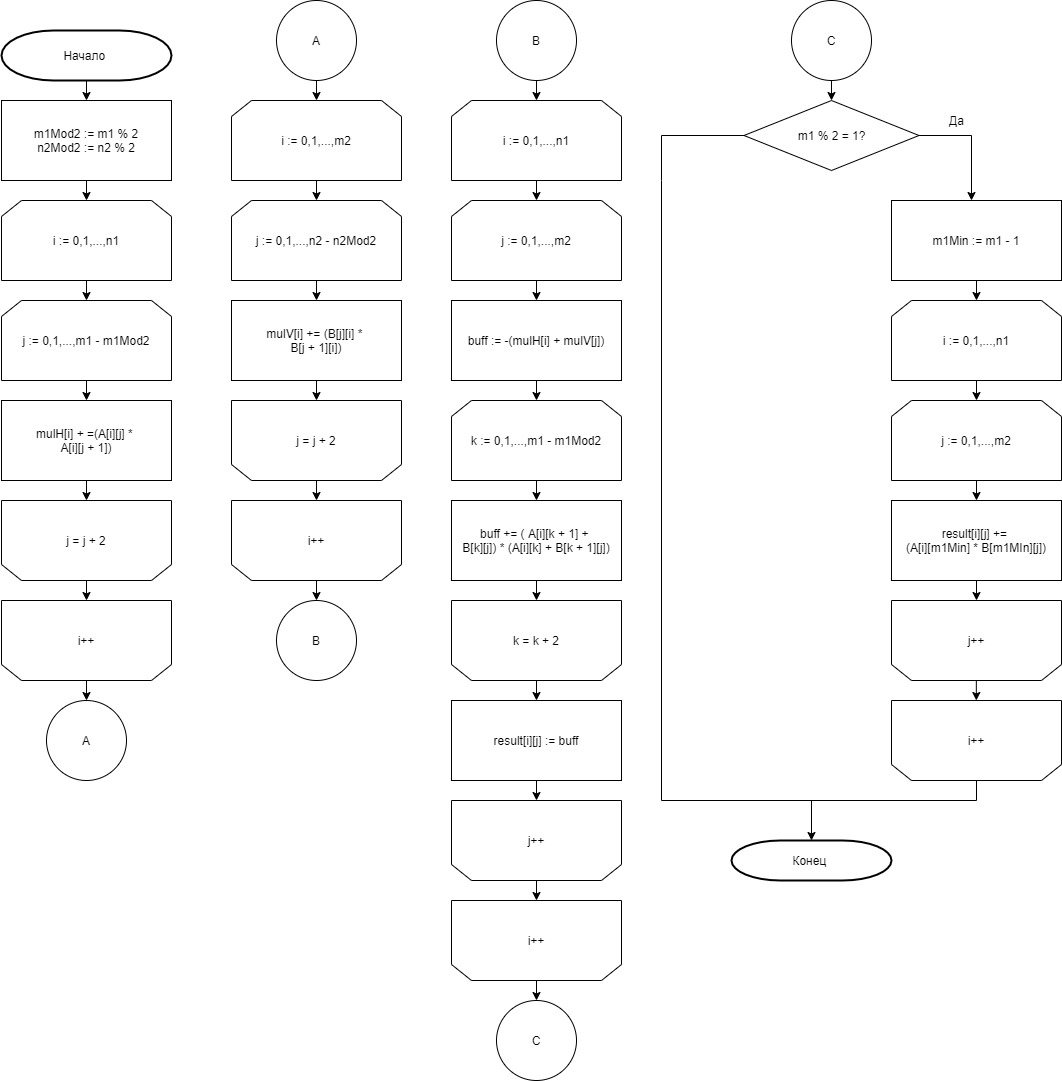
\includegraphics[width=1\linewidth]{src/schemas/vinograd_modified}\\
	Рис. 1.3: Схема улучшенного алгоритма Винограда
\end{center}
\addcontentsline{toc}{subsection}{Вывод}
\section*{Вывод}
\qquad В данном разделе были рассмотрены схемы реализуемых алгоритмов.
\clearpage


\section{Технологическая часть}
\qquad В данном разделе будет описана технологическая часть лабораторной работы: требования к ПО, листинг кода, сравнительный анализ всех алгоритмов.
\subsection{Требования к программному обеспечению}
Входные данные: Размерности двух матриц, сами матрицы.\\
\qquad Выходные данные: результат умножения двух матриц.\\
\qquad Среда выполнения: Windows 10 x64.\\
\subsection{Средства реализации}
\qquad Для выполнения данной лабораторной работы использовался ЯП Python 3.9.0
\subsection{Листинг кода}
\qquad В данном разделе будет представлен листинг кода разработанных алгоритмов (листинги 3.1 - 3.3).\\
\subsubsection{Обычный алгоритм умножения}
\qquad Ниже, на листинге 3.1,  представлена реализация обычного алгоритма умножения матриц:
\begin{center}
	Листинг 3.1: Обычный алгоритм умножения матриц
	\lstinputlisting[language=C++]{src/code/mult_trivial.cpp}
\end{center}
\clearpage

\subsubsection{Алгоритм Винограда}
\qquad Ниже, на листинге 3.2,  представлена реализация алгоритма Винограда:
\begin{center}
	Листинг 3.2: Алгоритм Винограда
	\lstinputlisting[language=C++]{src/code/vinograd_default.cpp}
\end{center}
\clearpage
\subsubsection{Улучшенный алгоритм Винограда}
\qquad Ниже, на листинге 3.3,  представлена реализация улучшенного алгоритма Винограда:
\begin{center}
	Листинг 3.3: Улучшенный алгоритм Винограда
		\lstinputlisting[language=C++]{src/code/vinograd_advanced.cpp}
\end{center}
\clearpage

\subsection{Сравнительный анализ обычного и улучшенного Алгоритма Винограда}
\qquad Улучшенный вариант алгоритма Винограда отличается от обычного тем, что теперь заранее высчитываются значения, для избавления от деления в цикле. А также инициализируется буфер для накопления результата умножения, который после цикла сбрасывается в ячейку матрицы.

\subsection{Трудоемкость алгоритмов}
\qquad Введем модель трудоемкости для оценки алгоритмов:\\
\begin{itemize}
\item базовые операции стоимостью 1: +, -, *, /, =, ==, <=, >=, !=, +=, [], получение полей класса (в том числе и геттеры);\\
\item оценка трудоемкости цикла: $F_{cycle} = init +  N*(statement + iteration + F_{body}) + statement$, где init - инициализация цилка, N - количество итераций цикла, iteration - действие в конце каждой итерации цикла, statement - выражение, описывающее условие цикла;\\
\item стоимость условного перехода применим за 0, стоимость вычисления условия остаётся.\\
\end{itemize}

\subsubsection{Классический алгоритм}
Рассмотрим трудоемкость классического алгоритма с матрицами A и B и размерами $m\times n$ и $n\times k$ : \\\\
$2 + M(2 + 2 + K(2 + 2 + N(2 + 6 + 2))) = 
10MNK + 4MK + 4M + 2 .
$

\subsubsection{Алгоритм Винограда}
Аналогично рассмотрим трудоемкость алгоритма Винограда при тех же матрицах и размерах.
\begin{table}[h]
\label{tabular:timesandtenses}
\begin{center}
\begin{tabular}{ l  l  }
    Часть алгоритма            & Трудоёмкость                                                        \\ \hline
    Инициализация mulH и mulV  & $2 \cdot 3$                                                         \\
    Заполнение mulH            & $2 + m \cdot (2 + 2 + n / 2 \cdot (3 + 6 + 6))$                     \\ 
    Заполнение mulV            & $2 + k \cdot (2 + 2 + n / 2 \cdot (3 + 6 + 6))$                     \\ 
    Подсчёт результата         & $2 + m \cdot (2 + 2 + k \cdot (2 + 7 + 2 + n / 2 \cdot (3 + 23)))$  \\ 
    Условный оператор нечёт. n & $2$                                                                 \\ 
    Для матриц с нечёт n       & $2 + m \cdot (2 + 2 + k \cdot (2 + 8 + 5))$                         \\ 
\end{tabular}
\caption{трудоёмкость алгоритма Винограда}  
\end{center}
\end{table}
\begin{displaymath}
    f = 13NMK + 7.5NM + 7.5KN + 11KM + 8M + 4K + 14 + \left \{ 
    \begin{array}{ll}  
        0, \textrm{если m чётное} \\ 
        15 \cdot K \cdot M + 4 \cdot M + 2, \textrm{иначе} 
    \end{array} \right.
\end{displaymath}

\subsubsection{Оптимизированный алгоритм Винограда}
Теперь рассмотрим трудоемкость оптимизированого алгоритма Винограда при тех же матрицах и размерах. 
\begin{table}[h]
  \label{tabular:timesandtenses}
\begin{center}
\begin{tabular}{  l  l  }
        Часть алгоритма               & Трудоёмкость                                                            \\ \hline
        Заполнение mulH               & $2 + m \cdot (2 + 2 + n / 2 \cdot (2 + 5 + 3))$                         \\ 
        Заполнение mulV               & $2 + k \cdot (2 + 2 + n / 2 \cdot (2 + 5 + 3))$                         \\ 
        Подсчёт результата            & $2 + m \cdot (2 + 2 + k \cdot (2 + 5 + 3 + 2  + n / 2 \cdot (2 + 14)))$                                             \\ 
        Условный оператор нечёт. n   & $2$                                                                     \\
        Для матриц с нечёт n          & $2 + 2 + m \cdot (2 + 2 + k \cdot (2 + 6 + 2))$                         \\ 
\end{tabular}
\caption{трудоёмкость оптимизированного алгоритма Винограда}
\end{center}
\end{table}
\begin{displaymath}
    f = 8NMK + 5NM + 5KN + 12KM + 8M + 4K + 18 + \left \{ 
    \begin{array}{ll}  
        0, \textrm{если m чётное} \\ 
        10 \cdot K \cdot M + 4 \cdot M + 4, \textrm{иначе} 
    \end{array} \right.
\end{displaymath}

\subsubsection{Описание тестирования} % описать, какие тесты будут проведены ВСЕ ТЕСТЫ ПРОЙДЕНЫ УСПЕШНО
Были проведены следующие тривиальные тесты:\\
\begin{lstlisting}[label=some-code,caption= Число строк равно числу стобцов]
A matrix:
1 2 
3 4

B matrix:
5 6
7 8  

Default multiplication:  
19 22
43 50

Winograd:
19 22
43 50

Improved Winograd:
19 22
43 50
\end{lstlisting}

\begin{lstlisting}[label=some-code,caption= Число строк равно числу стобцов]
A matrix:
1 2 3
4 5 6
7 8 9

B matrix:
1 2 3
4 5 6
7 8 9  

Default multiplication:  
30 36 42
66 81 96
102 126 150

Winograd:
30 36 42
66 81 96
102 126 150

Improved Winograd:
30 36 42
66 81 96
102 126 150
\end{lstlisting}

\qquad Ниже, на листинге 3.4, представлен листинг тестирования корректной работы алгоритмов.
\begin{center}
	Листинг 3.4: Тестирование корректной работы алгоритмов
	\lstinputlisting[language=C++]{src/code/random_matrices_tests.cpp}	
\end{center}
Все тесты пройдены успешно.\\
\addcontentsline{toc}{subsection}{Вывод}
\section*{Вывод}
\qquad В данном разделе был представлен листинг реализованных алгоритмов, а также описание тестирование корректности их работы.
\clearpage

\section{Экспериментальная часть}
\subsection{Сравнительный анализ на основе замеров времени работы алгоритмов}
Эксперименты производятся на квадратных матрицах размером от 100/101 x 100/101 до 500/501 x 500/501 c шагом 100. Эксперимент для каждой размерности матрицы проводится 10 раз, а итоговое время усредняется. Время работы алгоритмов измеряется в секундах.\\\\
\textbf{Сравнение времени работы алгоритмов при четном размере матрицы} \\
На графике изображены  зависимости времени выполнения программы от четного размера входных квадратных матриц: 
\begin{center}
График 1: Замеры времени работы алгоритмов
\begin{tikzpicture}
\begin{axis}[
axis lines = left,
xlabel = {Размер матрицы},
ylabel = {Время (с)},
legend pos=north west,
ymajorgrids=true ]
\addplot[color=red, mark=square] table[x index=0, y index= 1] {original.txt}; 
\addplot[color=green, mark=square] table[x index=0, y index= 1] {vinograd.txt}; 
\addplot[color=blue, mark=square] table[x index=0, y index= 1] {optim.txt}; 
\addlegendentry{Стандартный}
\addlegendentry{Виноград}
\addlegendentry{Оптимизированный}
\end{axis}
\end{tikzpicture}
\end{center}
\textbf{Сравнение времени работы алгоритмов при нечетном размере матрицы} \\
На графике изображены зависимости времени выполнения программы от нечетного размера входных квадратных матриц:  
\begin{center}
График 2: Замеры времени работы алгоритмов
\begin{tikzpicture}
\begin{axis}[
axis lines = left,
xlabel = {Размер матрицы},
ylabel = {Время (с)},
legend pos=north west,
ymajorgrids=true ]
\addplot[color=red, mark=square] table[x index=0, y index= 1] {original1.txt}; 
\addplot[color=green, mark=square] table[x index=0, y index= 1] {vinograd1.txt}; 
\addplot[color=blue, mark=square] table[x index=0, y index= 1] {optim1.txt}; 
\addlegendentry{Стандартный}
\addlegendentry{Виноград}
\addlegendentry{Оптимизированный}
\end{axis}
\end{tikzpicture}
\end{center}
\clearpage
\section*{Вывод}
\qquad По результатам тестирования все рассматриваемые алгоритмы реализованы так, что возвращают одинаковый результат. Самым медленным алгоритмом оказался алгоритм классического умножения матриц, а самым быстрым — оптимизированный алгоритм Винограда.
\clearpage
\addcontentsline{toc}{section}{Заключение}
%//////////////////////////////////////////////////////////////////
\section*{\Huge Заключение}
Цель достигнута и все задачи выполнены. \\\\
В ходе работы были изучены  и реализованы алгоритмы умножения матриц: классический алгоритм, алгоритм Винограда, улучшенный алгоритм
Винограда. Была дана теоретическая оценка всех рассматриваемых алгоритмов, было проведено тестирование и выполнено сравнение всех рассматриваемых алгоритмов. В ходе исследования было установлено, что улучшенный алгоритм Винограда является самым быстрым алгоритмом по трудоемкости и времени выполнения среди рассмотренных алгоритмов умножения матриц. Изучены зависимости времени выполнения алгоритмов от размерности матриц.

\clearpage

\begin{thebibliography}{}
	\bibitem{}  Дж. Макконнелл. Анализ алгоритмов. Активный обучающий подход. – М.: Техносфера, 2017. – 267с
	\bibitem{}  Кострикин А.И., Манин Ю.И. Линейная алгебра и геометрия. -- СПб: Лань, 2018. --\\ 303 с.
	\bibitem{python}Официальный сайт Python, документация [электронный ресурс]. Режим доступа: https://docs.python.org/3.9, свободный – (Дата обращения: 8.10.20)
\end{thebibliography}

\end{document}